%% ----- INTRODUCTION -----
\section{Introduction}
\label{pave-intro}

Building on the initial success of COVID-Sim and the subsequent AVOEV project website described in Chapter \ref{ch:avov}, this chapter describes a third and final project-specific portal built using the same combination of curated runs stored on a file server and a custom front-end website. This project website was intended to be outward-facing, for public outreach meetings with government agencies and the wider public audience, rather than an internal-facing analyst tool.

%% ----- PROJECT DESCRIPTION -----
\section{Project Description}
\label{pave-project-description}

The \gls{PAVE} project studied the ``Potential of Automated Transport Systems'' in Berlin, Germany, and concluded its research in 2022. The project team was comprised of a consortium of multiple universities and private firms in Germany.\footnote{To learn more about the PAVE Project and PAVE Consortium, see the main PAVE website at \href{https://pave-your-way.de}{pave-your-way.de}}

The project explores several demand-responsive transport (\gls{DRT}) configurations including automated taxi service (``Robotaxi''), automated, pooled shuttle service (``Pooling''), combinations of these services, as well as a strict ban on non-DRT private vehicles inside Berlin. Multiple service areas, cost structures, fleet sizes, and several other parameters are studied.

\subsection{DRT scenarios being studied}
\label{pave-scenarios}

While the study details themselves are not critical, a basic overview of the scenarios being tested is helpful to understand how the data visualizations for the project website are constructed.

These four main scenarios are being considered:

\textbf{Robotaxi.} In this scenario, one passenger at a time can be transported by each DRT vehicle. The DRT provider aims to minimize the needed subsidy (or maximize profit) while trying to hold 95 percent of wait times to 7 minutes or below; this can be seen as a regulatory constraint. The simulation was used to approximate the resulting demand and the necessary fleet size for several cost structure alternatives at a rough planning level.

\textbf{Pooling.} In this scenario, multiple passengers can be transported by each DRT vehicle simultaneously. In this scenario the DRT provider also aims to minimize the needed subsidy need (or maximize profit),  while trying to keep 95 percent of wait times below 7 minutes. The simulation was used to approximate the fleet size needed and the resulting demand for various user prices. The base fare is paid per ride; the price per km is paid for the direct distance when booking the ride. When several passengers get pooled the actual travelled distance may differ.

\textbf{Combined.} In this scenario, travelers can choose between both mobility-on-demand modes of operation. The ``robotaxi'' service is operated within the inner core of Berlin, while the pooling service area covers the entire city. The taxi operator is more expensive as it guarantees direct transportation. As in the robotaxi and pooling scenarious above, the simulation approximated the resulting demand and necessary fleet sizes, but in this case for both operators in competition with each other.

\textbf{Ban private vehicles.} In this scenario, private cars are banned from the inner core of Berlin. As a substitute, a DRT system is introduced. People can transfer from their private cars to the DRT system and vice-versa, which happens at the border of the car-free zone. No regulatory waiting time threshold is assumed in this scenario.

%% ----- UNIQUE SITE FEATURES -------------------------------
\section{Supporting decisionmaking with an interactive website}
\label{pave-site-features}

To support the public outreach meetings for the PAVE project, a third project-specific website was built using a similar technology stack as for the previously described COVID-Sim and AVOEV projects. This site is available online at \url{https://vsp.berlin/pave}. The goal was to build something that agency staff and the genuine public could use, therefore a much larger effort was spent on honing the user interface and usability of the site; for example, paying more attention to creating a pleasing layout and a consistent color palette, and also including explanatory text where needed to avoid overly technical jargon.

Roadway volume plots, simulated DRT vehicle animations, and mode shift charts similar to those used in the AVOEV project were implemented for the PAVE website. These are described in sections \ref{avov-drtviz} and \ref{avov-volumes}.

Some new and updated components were built, and these are described below.

%% ----- -----------------------------------
\subsection{Scenario chooser}
\label{pave-scenario-chooser}

Building on the multivariate COVID-Sim simulation result picker described in section \ref{covid-single-page-application}, a new scenario chooser was built for PAVE. An iterative procedure for improving the design and features, working closely with the analyst team, led to the final layout and behavior. Large graphical elements depicted the different service areas on a map, along with buttons for selecting differing fare structures. The user could essentially browse and select from the various scenarios shown on a left-side navigation panel, and the results for that scenario would immediately appear in the main window pane.

Figure \ref{fig:pave-scenario-chooser} shows a close-up of a typical scenario output page, with the scenario selector on the left side and the various outputs to the right. These are explained in more detail below.

\begin{figure}[ht]
  \centering
  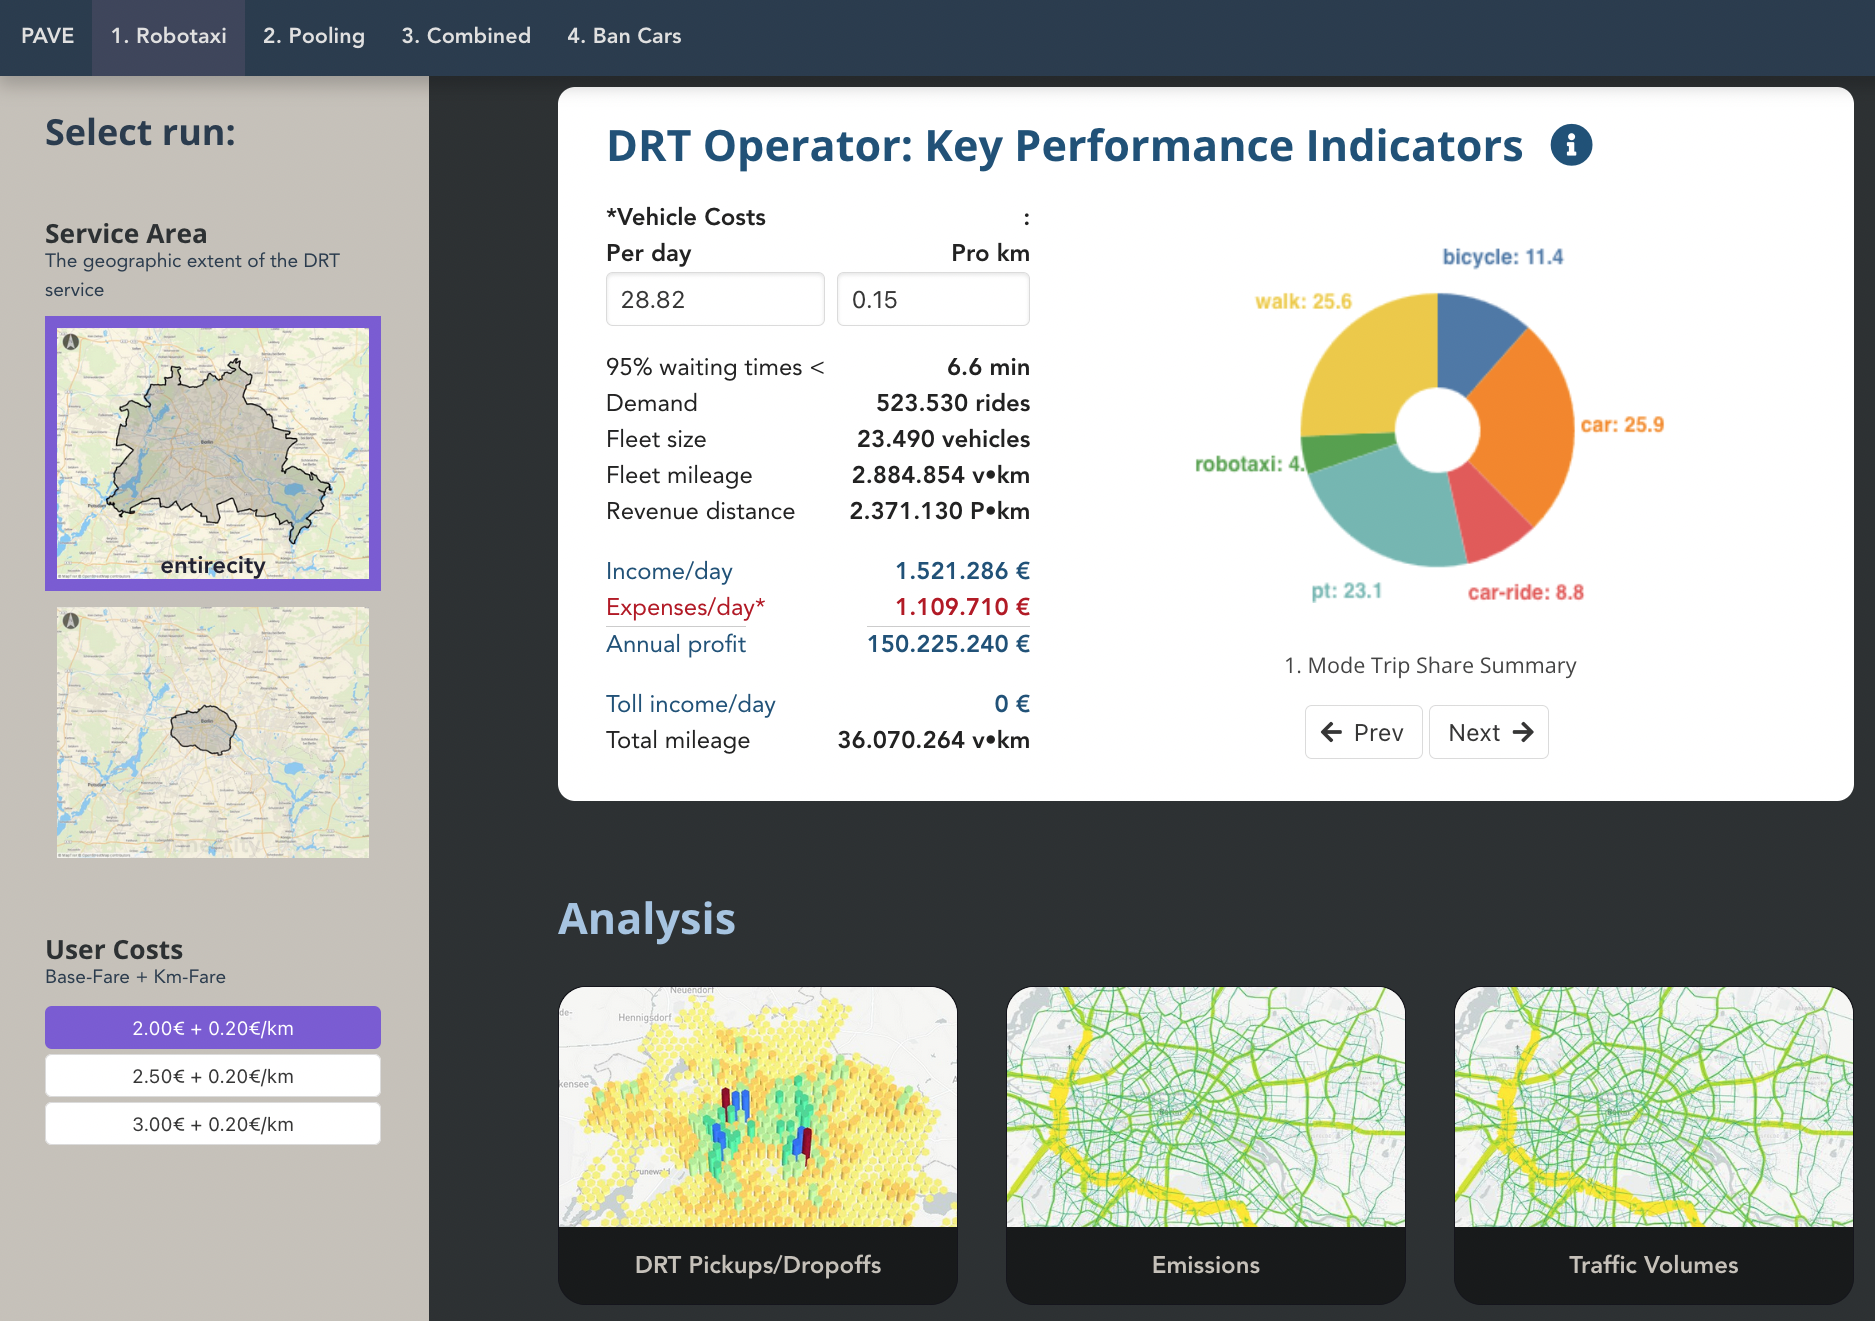
\includegraphics[width=0.95\linewidth]{chapters/23-pave/images/fig-kpi-panel.png}
  \caption{Screenshot of PAVE scenario viewer, with left-side selector and key performance indicators and visualizations on the right}
  \label{fig:pave-scenario-chooser}
\end{figure}

%% ----- -----------------------------------
\subsection{Key performance indicator panel}
\label{pave-kpi-panel}

A new summary \gls{KPI} panel provided top-level summary statistics for the selected scenario. This panel went through many rounds of revision with the analyst team and project partners before settling on the final set of KPIs. The panel includes aggregate statistics including total demand, fleet size, fleet mileage, operator income and expenses, and also includes a ``carousel'' of mode share and mode shift diagrams which the user can scroll through.

This KPI panel also includes interactive text entry fields for vehicle costs, both per-vehicle and per-km, so that users can explore the consequences of different cost parameters if they desire. Default values are used initially, but any cost parameters can be tested in this manner

Figure \ref{fig:pave-scenario-chooser} includes an example of the KPI panel.

%% ----- -----------------------------------
\subsection{Interactive DRT animation}
\label{pave-drt-animation}

The DRT animation plugin from the AVOEV project (see Section \ref{avov-drtviz}) was updated and improved for the PAVE project. Much larger simulation support was added, as the PAVE project encompasses the capital city of Berlin instead of less-populated rural areas of Germany, as in AVOEV.

This support was enabled by use of the JavaScript \emph{crossfilter} library.\footnote{Crossfilter is available online at \href{https://crossfilter.github.io/crossfilter/}{crossfilter.github.io/crossfilter/}} Crossfilter allows filtering and exploring of large multivariate datasets, and supports extremely fast (measured in milliseconds) interaction with coordinated views, even with datasets containing millions of records. Crossfilter takes advantage of the fact that most user interactions only modify a single dimension at a time (in this case the elapsed time of the simulation), which requires only small adjustments to filter values. Incremental filtering and reducing is significantly faster than starting from scratch. Crossfilter uses sorted numerical indexes, dramatically increasing perfor­mance over other sorting and filtering techniques.

With this library, the vehicle position dataset can be filtered to include only the exact second of the simulation that is currently displayed, and then only those filtered vehicle trace segments are painted on the screen. Up to tens of thousands of vehicles can be simultaneously animated in the browser using this technique.

For example screenshots of the DRT animation, refer to Figure \ref{fig:avov-drt-vehicles-routes}.

Note that for even larger datasets, crossfilter was no longer sufficient and more direct graphical methods using \gls{GPU} accelerated techniques were required. Those techniques are addressed in Chapter \ref{ch:simwrapper}.

%% ----- -----------------------------------
\subsection{Aggregate DRT origin/destination patterns}
\label{pave-od-hexagons}

An aggregate summary of the origin and destination locations of DRT trips was also created to help show the ``big picture'' of how DRT was being used in the study area; individual vehicle animations described above are very visually pleasing but do not provide a comprehensive systemic depiction.

Often, this type of aggregate summary data is collected into districts or analysis ``zones'' that are predetermined by analysts. For this visualization, a fully interactive plot was implemented consisting of hexagonal areas equally distributed across the study area; and the size of the hexagons themselves is user-selectable with a simple slider.

The hexagon plot aggregates either total DRT trips originating or destined for points inside each hexagon; the aggregation is then colored from pale to dark to emphasize areas with large numbers of DRT trips. A three-dimensional view is also possible, with the total aggregate value mapped to the height of hexagonal ``cylinders'' on the map.

An example of this hexagon-area-based DRT trip aggregation is shown in Figure \ref{fig:pave-xy-origins}, showing an example of total DRT trip origins.

\begin{figure}[ht]
\centering
  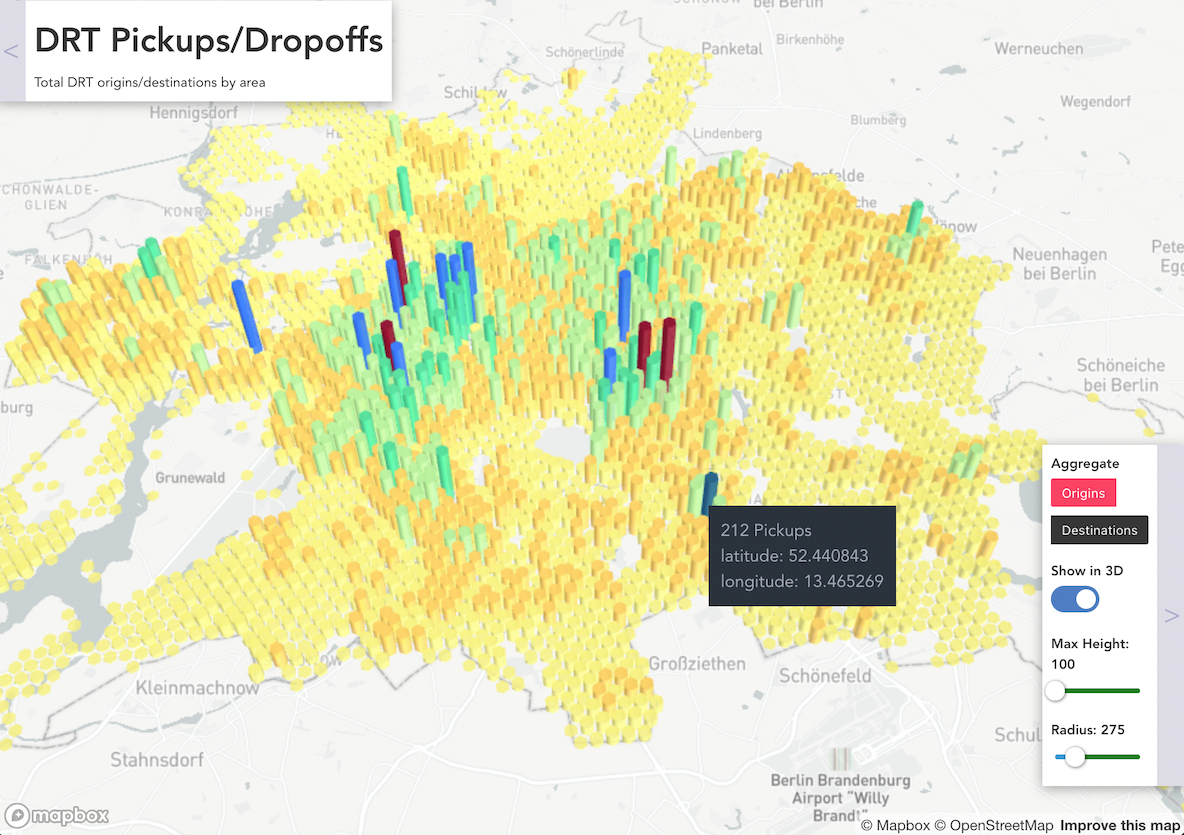
\includegraphics[width=0.95\linewidth]{chapters/23-pave/images/fig-xy-origins.png}
\caption{PAVE aggregate summary of DRT trip origins for an example scenario. Color and height represent the total number of trips in an area, and the user can hover over an area to see the precise number of trips.}
\label{fig:pave-xy-origins}
\end{figure}

%% ----- FEEDBACK -----
\section{Public Outreach Results and Feedback}
\label{pave-feedback}

The website was introduced to consortium partners and was presented to the public in multiple public outreach meetings in Berlin during spring 2021. Staff used the site to explain to the public how the different scenarios were configured, and then participants were given the opportunity to explore the site on their own, while also examining more traditional outreach materials including handouts and posters.

Feedback from staff was generally positive: one team member stated, ``I think people liked it. But mostly they wanted to talk to us about the different scenarios and interact with us directly, instead of using the website.''

%% ----- DISCUSSION AND OUTLOOK -----
\section{Discussion and Outlook}
\label{pave-discussion}

As the visualization platform for these project websites grows in capability, its usefulness to analysts grows as well. However, the level of effort to produce a website portal for this one small project was unacceptably high: the site was built over the course of three months and many hours were spent making small modifications on an iterative basis. Some new components that were developed have potential to be used in future projects, but that would require that the components be made in a more modular fashion that is not tied to specific project outputs.

Overall, the built site was well-received in the public outreach sessions and was well-liked by analyst staff. To truly inform the public and the decisionmaking process requires more than pleasing maps or a nice website, but it did appear to have a positive impact on discussions, however small.

The PAVE project was the third project site built on a common foundation of web-based visualization technologies and HTTP-accessible file storage for site configuration and simulation outputs. Several novel components were built for the project, including visual navigation for scenario selection, a consistent key performance indicator output panel, three-dimensional interactive display of trip origin and destination patterns, and a carousel for collating related charts in order to reduce visual clutter.

Feedback from users and internal staff was positive. In fact, the team at VSP felt that the overall concept had been more than adequately proven, and wanted to include the development of browser-based interactive visualizations in future proposals for publicly-funded projects. Despite this enthusiasm, the level of effort to produce this project site was much higher than desired. There were suggestions that the core features might be better integrated in a \emph{general visualiztion platform} instead of creating additional project-specific websites. The development of a generic data visualization platform in this vein is the subject of the following chapters, in Part III.
